\begin{frame}{$^3He(K^-, d) w/ \pi^+ \pi^-$ events}
  \centering
  $^3He(K^-, d \pi^+ \pi^-)"n"$ events was clearly seen. \\
  $^3He(K^-, d \pi^+)"\Sigma^-$ and $^3He(K^-, d \pi^-)"\Sigma^+$ were clearly seen.\\
  $K^0$ events was clearly seen.\\
  \begin{tabular}{cc}
    \begin{minipage}{0.5\hsize}
      \begin{figure}
        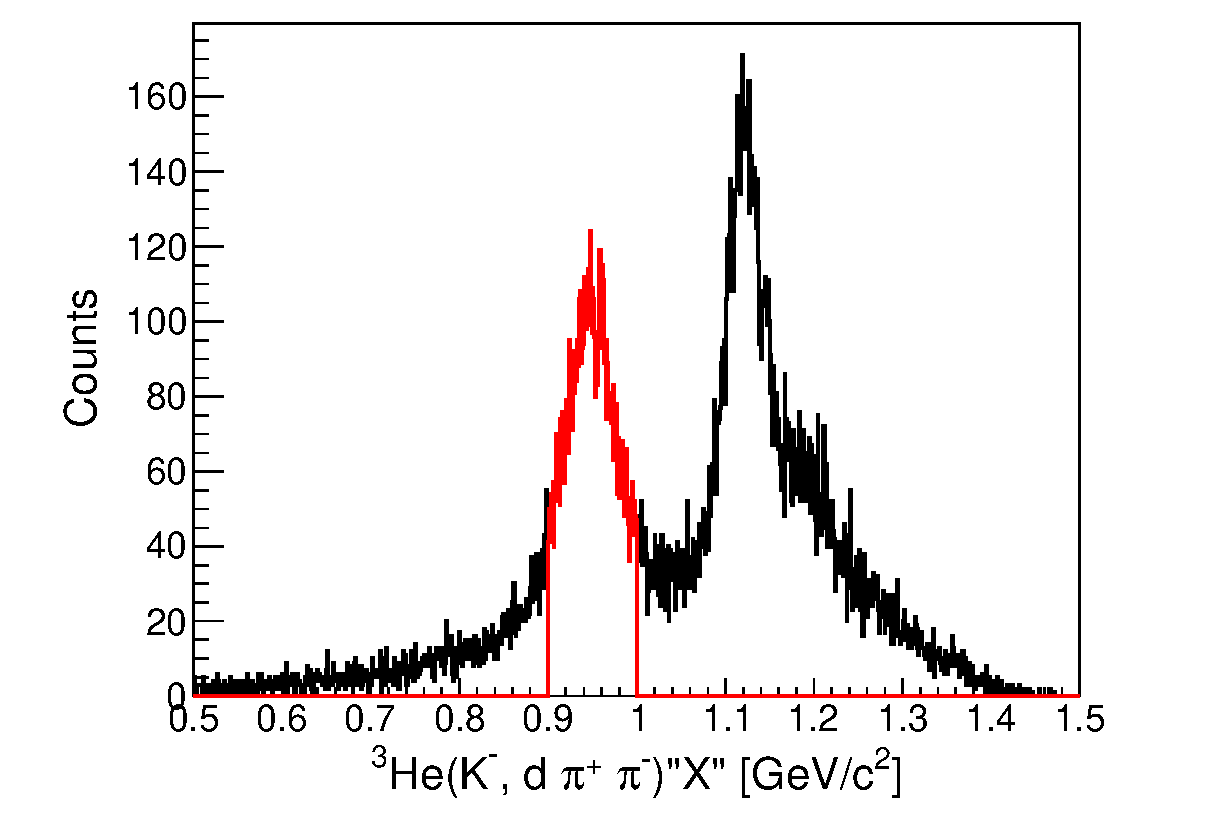
\includegraphics[width=4cm]{../pic/Run65/KDpipi_MM.eps}
      \end{figure}
    \end{minipage}

    \begin{minipage}{0.5\hsize}
      \begin{figure}
        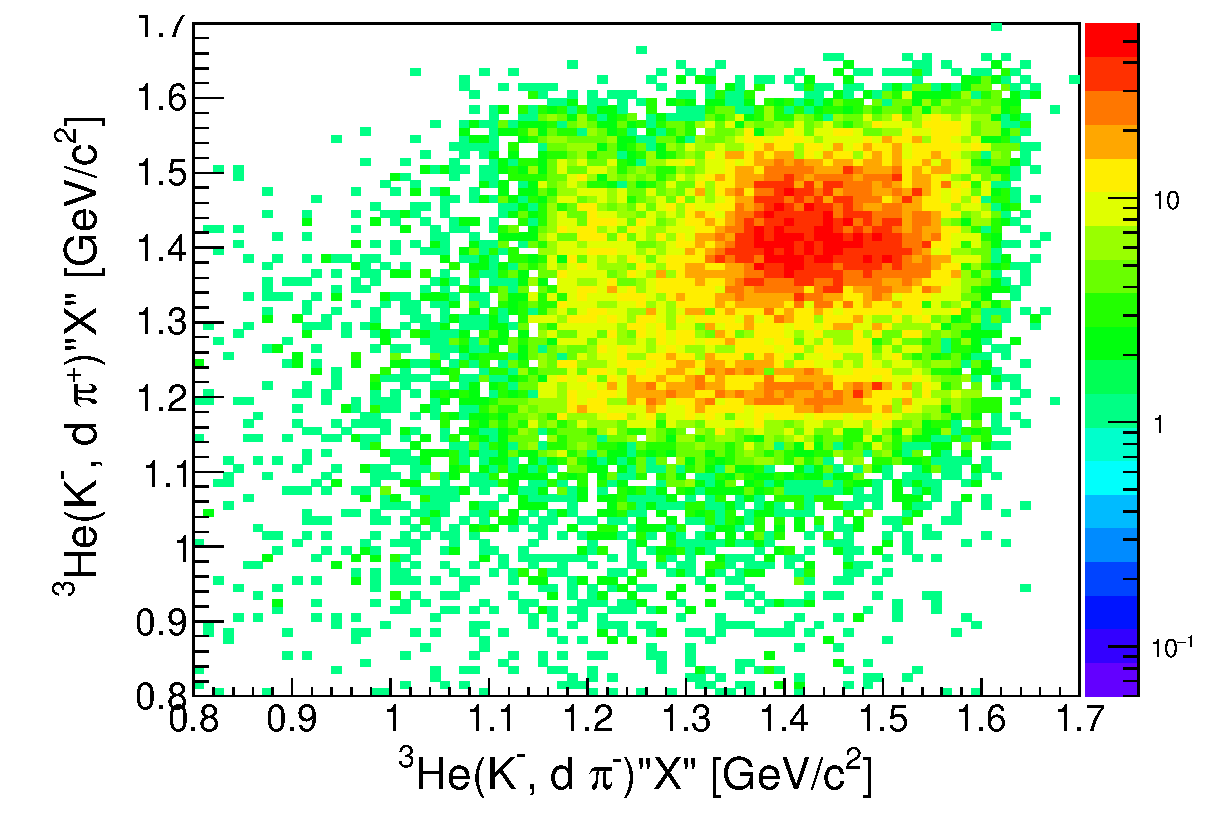
\includegraphics[width=4cm]{../pic/Run65/KDpim_KDpip_MM.eps}
      \end{figure}      
    \end{minipage}
  \end{tabular}


  \begin{tabular}{cc}
    \begin{minipage}{0.5\hsize}
      \begin{figure}
        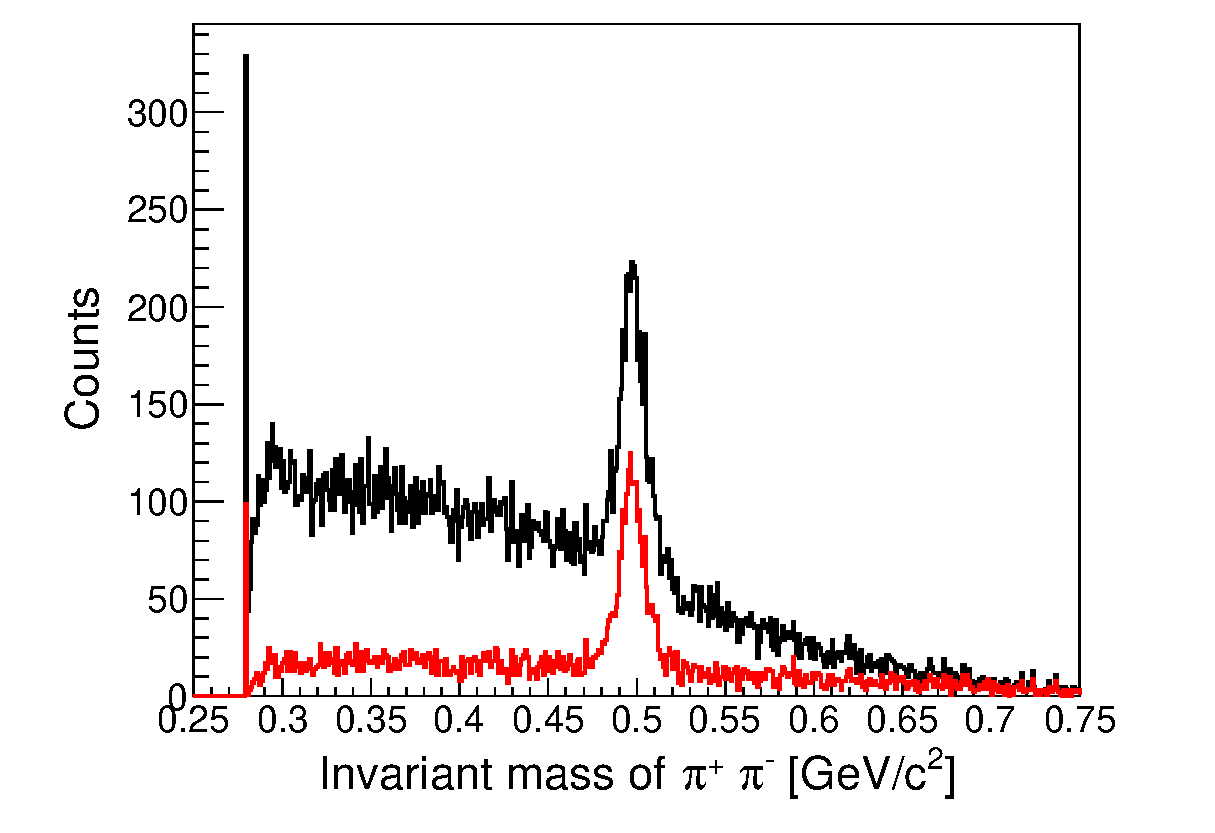
\includegraphics[width=4cm]{../pic/Run65/pipi_IM_wD.eps}
      \end{figure}
    \end{minipage}

    \begin{minipage}{0.5\hsize}
      \begin{figure}
        $^3He(K^-, d \pi^+ \pi^-)"n"$ select
        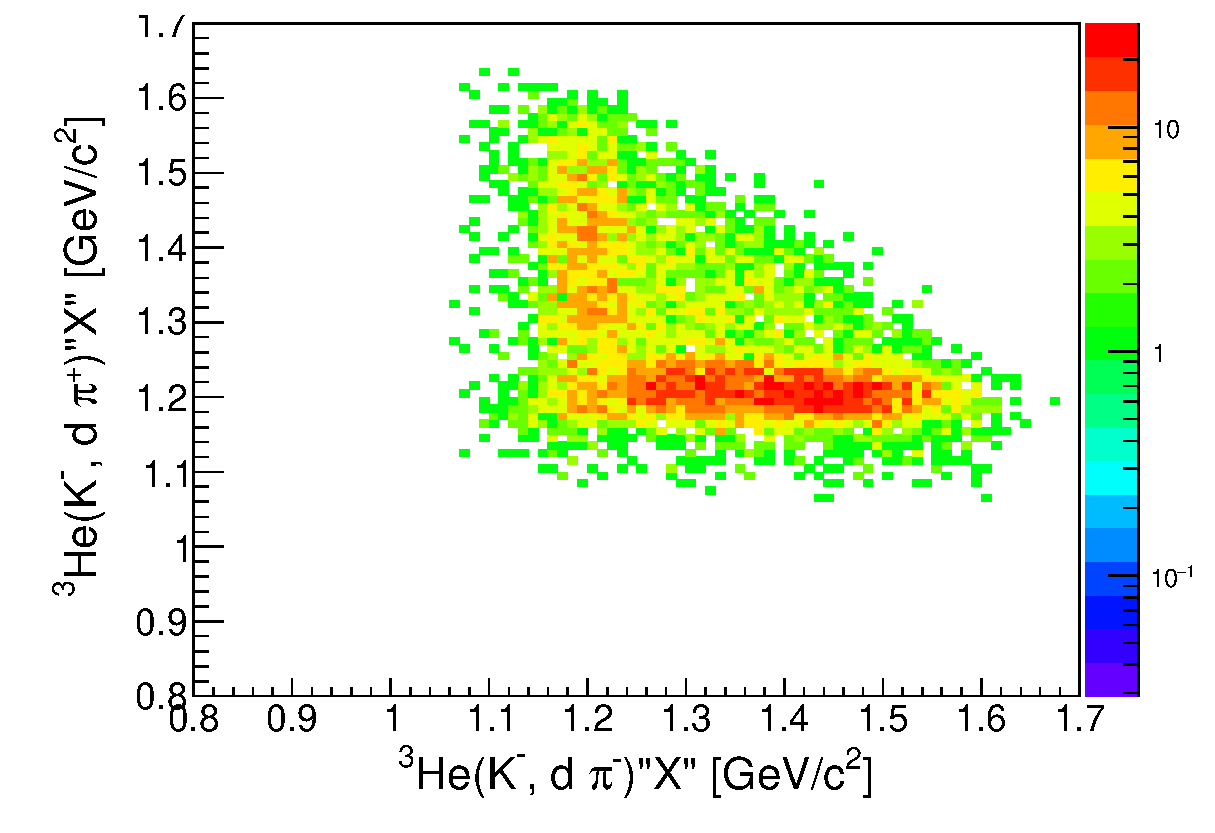
\includegraphics[width=4cm]{../pic/Run65/KDpim_KDpip_MM_mmN.eps}
      \end{figure}      
    \end{minipage}
  \end{tabular}
\end{frame}
